\documentclass[journal,12pt,twocolumn]{IEEEtran}
\usepackage{setspace}
\usepackage{gensymb}
\singlespacing
\usepackage[cmex10]{amsmath}
\usepackage{amsthm}
\usepackage{mathrsfs}
\usepackage{txfonts}
\usepackage{stfloats}
\usepackage{bm}
\usepackage{cite}
\usepackage{cases}
\usepackage{subfig}
\usepackage{longtable}
\usepackage{multirow}
\usepackage{enumitem}
\usepackage{mathtools}
\usepackage{tikz}
\usepackage{circuitikz}
\usepackage{verbatim}
\usepackage[breaklinks=true]{hyperref}
\usepackage{tkz-euclide} % loads  TikZ and tkz-base
\usepackage{listings}
\usepackage{color}    
\usepackage{array}    
\usepackage{longtable}
\usepackage{calc}     
\usepackage{multirow} 
\usepackage{hhline}   
\usepackage{ifthen}   
\usepackage{lscape}     
\usepackage{chngcntr}
\DeclareMathOperator*{\Res}{Res}
\renewcommand\thesection{\arabic{section}}
\renewcommand\thesubsection{\thesection.\arabic{subsection}}
\renewcommand\thesubsubsection{\thesubsection.\arabic{subsubsection}}

\renewcommand\thesectiondis{\arabic{section}}
\renewcommand\thesubsectiondis{\thesectiondis.\arabic{subsection}}
\renewcommand\thesubsubsectiondis{\thesubsectiondis.\arabic{subsubsection}}
\renewcommand\thetable{\arabic{table}}
% correct bad hyphenation here
\hyphenation{op-tical net-works semi-conduc-tor}
\def\inputGnumericTable{}                                 %%

\lstset{
%language=C,
frame=single, 
breaklines=true,
columns=fullflexible
}
%\lstset{
%language=tex,
%frame=single, 
%breaklines=true
%}

\begin{document}
\newtheorem{theorem}{Theorem}[section]
\newtheorem{problem}{Problem}
\newtheorem{proposition}{Proposition}[section]
\newtheorem{lemma}{Lemma}[section]
\newtheorem{corollary}[theorem]{Corollary}
\newtheorem{example}{Example}[section]
\newtheorem{definition}[problem]{Definition}
\newcommand{\BEQA}{\begin{eqnarray}}
\newcommand{\EEQA}{\end{eqnarray}}
\newcommand{\define}{\stackrel{\triangle}{=}}
\bibliographystyle{IEEEtran}
\providecommand{\mbf}{\mathbf}
\providecommand{\pr}[1]{\ensuremath{\Pr\left(#1\right)}}
\providecommand{\qfunc}[1]{\ensuremath{Q\left(#1\right)}}
\providecommand{\sbrak}[1]{\ensuremath{{}\left[#1\right]}}
\providecommand{\lsbrak}[1]{\ensuremath{{}\left[#1\right.}}
\providecommand{\rsbrak}[1]{\ensuremath{{}\left.#1\right]}}
\providecommand{\brak}[1]{\ensuremath{\left(#1\right)}}
\providecommand{\lbrak}[1]{\ensuremath{\left(#1\right.}}
\providecommand{\rbrak}[1]{\ensuremath{\left.#1\right)}}
\providecommand{\cbrak}[1]{\ensuremath{\left\{#1\right\}}}
\providecommand{\lcbrak}[1]{\ensuremath{\left\{#1\right.}}
\providecommand{\rcbrak}[1]{\ensuremath{\left.#1\right\}}}
\theoremstyle{remark}
\newtheorem{rem}{Remark}
\newcommand{\sgn}{\mathop{\mathrm{sgn}}}
\providecommand{\abs}[1]{\left\vert#1\right\vert}
\providecommand{\res}[1]{\Res\displaylimits_{#1}} 
\providecommand{\norm}[1]{\left\lVert#1\right\rVert}
\providecommand{\mtx}[1]{\mathbf{#1}}
\providecommand{\mean}[1]{E\left[ #1 \right]}
\providecommand{\fourier}{\overset{\mathcal{F}}{ \rightleftharpoons}}
\providecommand{\system}[1]{\overset{\mathcal{#1}}{ \longleftrightarrow}}
\newcommand{\solution}{\noindent \textbf{Solution: }}
\newcommand{\cosec}{\,\text{cosec}\,}
\providecommand{\dec}[2]{\ensuremath{\overset{#1}{\underset{#2}{\gtrless}}}}
\newcommand{\myvec}[1]{\ensuremath{\begin{pmatrix}#1\end{pmatrix}}}
\newcommand{\mydet}[1]{\ensuremath{\begin{vmatrix}#1\end{vmatrix}}}
\renewcommand{\vec}[1]{\boldsymbol{\mathbf{#1}}}
\def\putbox#1#2#3{\makebox[0in][l]{\makebox[#1][l]{}\raisebox{\baselineskip}[0in][0in]{\raisebox{#2}[0in][0in]{#3}}}}
     \def\rightbox#1{\makebox[0in][r]{#1}}
     \def\centbox#1{\makebox[0in]{#1}}
     \def\topbox#1{\raisebox{-\baselineskip}[0in][0in]{#1}}
     \def\midbox#1{\raisebox{-0.5\baselineskip}[0in][0in]{#1}}
\vspace{3cm}
\title{PT-100 Lab Assignment}
\author{Nithish}
\maketitle
\tableofcontents
\bigskip
\begin{abstract}
    This document contains a lab report on the modeling of the voltage-temperature
    characteristics of the PT-100 RTD (Resistance Temperature Detector) using
    least squares method.
\end{abstract}
\section{Training Data}
The training data gathered by the PT-100 to train the Arduino is shown in the following table.
\begin{table}[!ht]
    \centering
    %%%%%%%%%%%%%%%%%%%%%%%%%%%%%%%%%%%%%%%%%%%%%%%%%%%%%%%%%%%%%%%%%%%%%%
%%                                                                  %%
%%  This is a LaTeX2e table fragment exported from Gnumeric.        %%
%%                                                                  %%
%%%%%%%%%%%%%%%%%%%%%%%%%%%%%%%%%%%%%%%%%%%%%%%%%%%%%%%%%%%%%%%%%%%%%%

\begin{center}
\begin{tabular}{|c|c|}
\hline
	\textbf{Temperature(in Celcius)}& \textbf{Voltage(in Volts)}\\ \hline
	24	&2.40	\\ \hline
	38	&2.44	\\ \hline
	45	&2.45   \\ \hline
	52	&2.48   \\ \hline
	63	&2.49   \\ \hline
	93	&2.55	\\ \hline
	100	&2.57	\\ \hline
\end{tabular}
\end{center}

    \caption{Training data}
    \label{tab:train}
\end{table}

\begin{figure}[!ht]
    \centering
    \begin{circuitikz} \draw
        (0,0) to[battery1, l=$3.3\ V$, invert] (0,2)
        to[R, l^=$50\ \Omega$] (3,2) to[short, -o] (5,2);
        \draw (3,2) to[R, l^=$P\ \Omega$] (3,0)
        -- (0,0);
        \draw (3,0) to[short, -o] (5,0);
    \end{circuitikz}
    \caption{Circuit Diagram}
    \label{fig:1}
\end{figure}

\section{Model}
For the PT-100, we use the Callendar-Van Dusen equation
\begin{align}
    V(T) &= \brak{C+BT+AT^2} \\
    \implies c &= \vec{x}^\top\vec{n} 
\end{align}
where
\begin{align}
    c = V(T),\ \vec{n} = \myvec{C\\B\\A},\ \vec{x} = \myvec{1\\T\\T^2}
\end{align}
For multiple points, the above equation becomes
\begin{align}
    \vec{X}^\top\vec{n} = \vec{c}
\end{align}
where
\begin{align}
    \vec{X} &= \myvec{1&1&\ldots&1\\T_1&T_2&\ldots&T_n\\T_1^2&T_2^2&\ldots&T_n^2} \\
    \vec{C} &= \myvec{V\brak{T_1}\\V\brak{T_2}\\\vdots\\V\brak{T_n}}
\end{align}
and $\vec{n}$ is the unknown.
\section{Solution}
We approximate $\vec{n}$ by finding the least squares estimate of it. The least square estimate of $\vec{n}$ for the above training data is

\begin{align}
	\vec{n} = \myvec{2.3348\\2.9394\times10^{-3}\\-6.2462\times10^{-6}}
\end{align}
The approximation is shown in Fig. 2, we can see that our model fits the training data very well.
\begin{figure}[!ht]
    :\centering
    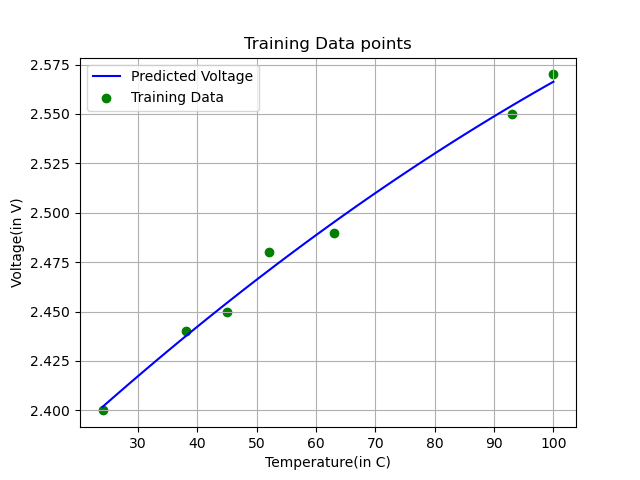
\includegraphics[width=\columnwidth]{figs/Training_Data.png}
    \caption{Training the model.}
    \label{fig:train}
\end{figure}
Thus, the approximate model is given by
\begin{align}
    V(T) &= 2.3348 + \brak{2.9394\times10^{-3}}T \nonumber \\
         &- \brak{6.2462\times10^{-6}}T^2
    \label{eq:opt-model}
\end{align}

\section{Validation}
The validation dataset is shown in Table 2. The results of the 
validation are shown in Fig. 3. We can see that our model perform well in validation data.

\begin{table}[!ht]
    \centering
    %%%%%%%%%%%%%%%%%%%%%%%%%%%%%%%%%%%%%%%%%%%%%%%%%%%%%%%%%%%%%%%%%%%%%%
%%                                                                  %%
%%  This is a LaTeX2e table fragment exported from Gnumeric.        %%
%%                                                                  %%
%%%%%%%%%%%%%%%%%%%%%%%%%%%%%%%%%%%%%%%%%%%%%%%%%%%%%%%%%%%%%%%%%%%%%%

\begin{center}
\begin{tabular}{|c|c|}
\hline
	\textbf{Temperature(in Celcius)}& \textbf{Voltage(in Volts)}\\ \hline
	29	&2.41	\\ \hline
	32	&2.43	\\ \hline
	74	&2.52   \\ \hline
	85	&2.54   \\ \hline
\end{tabular}
\end{center}

    \caption{Validation data.}
    \label{tab:valid}
\end{table}

\begin{figure}[!ht]
    \centering
    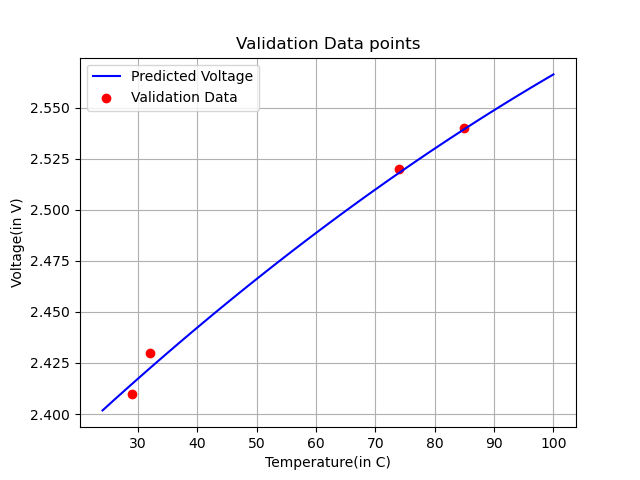
\includegraphics[width=\columnwidth]{figs/Validation_Data.png}
    \caption{Validating the model.}
    \label{fig:valid}
\end{figure}

\section{Conclusion}
In this project we saw how we can use simple machine learning techniques to map the characteristics of an unknown sensor. We also learned how we can idetinfy the temperature using a temperature dependent resistor like PT-100.
\end{document}
